\section{Extensions of Turing Machine}
\label{sec:exten-of-tm}

\subsection{Multiple Tapes}

One can think of Turing machines that have several tapes (see Figure 9). Each tape is connected to the finite control by means of a read/write head (one on each tape). The machine can in one step read the symbols scanned by all its heads and then, depending on those symbols and its current state, rewrite some of those scanned squares and move some of the heads to the left or right, in addition to changing state.

For any fixed integer $k \geq 1$, a $k$-tape Turing machine is a Turing machine equipped as above with $k$ tapes and corresponding heads. Thus a ``standard'' Turing machine studied so far in this chapter is just a $k$-tape Turing machine, with $k = 1$.
\begin{figure}[H]
  \centering
  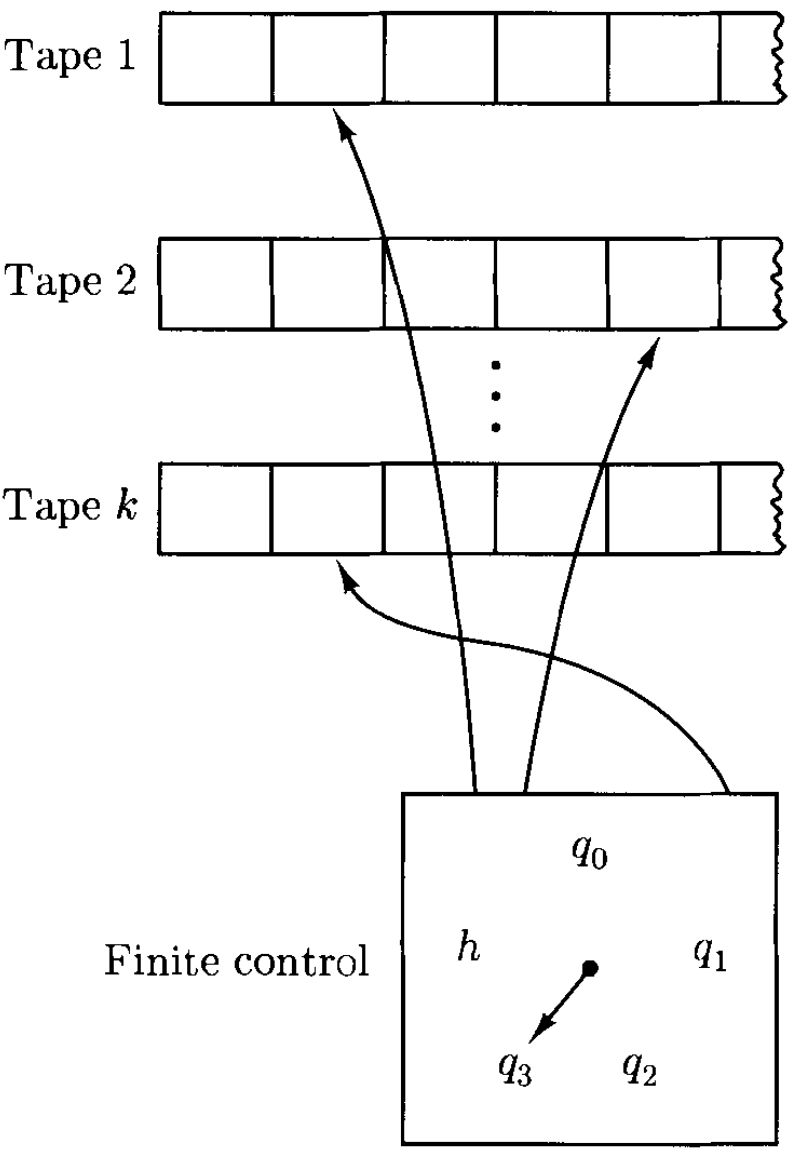
\includegraphics[width=.9\linewidth]{img/fig-4.14.png}
  \caption{}
  \label{fig:4.9}
\end{figure}

\vspace*{\fill}
\columnbreak

\begin{definition}{}
  Let $k \geq 1$ be an integer. A \textbf{$k$-tape Turing machine} is a quintuple $(K, \Sigma, \delta, s, H)$, where $K$, $\Sigma$, $s$, and $H$ are as in the definition of the ordinary Turing machine, and $\delta$, the \textbf{transition function}, is a function from $(K - H) \times \Sigma^k$ to $K \times (\Sigma \cup \{ \la, \ra \})^k$. That is, for each state $q$, and each $k$-tuple of tape symbols $(a_1, \ldots, a_k)$; $\delta(q,\ (a_1, \ldots, a_k)) = (p,\ (b_1, \ldots, b_k))$, where $p$ is, as before, the new state, and $b_j$ is, intuitively, the action taken by $M$ at tape $j$. Naturally, we again insist that if $a_j =\ \tar$ for some $j \leq k$, then $b_j = \ra$. 
\end{definition}
Computation takes place in all $k$ tapes of a $k$-tape Turing machine. Accordingly, a \textit{configuration} of such a machine must include information about all 
tapes:
\begin{definition}{}
Let $M = (K, \Sigma, \delta, s, H)$ be a $k$-tape Turing machine. A configuration of $M$ is a member of
\begin{equation*}
  K \times ( {\tar}{\Sigma^*} \times (\Sigma^* (\Sigma - \{\blank\}) \cup \{ e \}))^k
\end{equation*}
That is, a configuration identifies the \textit{state}, the \textit{tape contents}, and the \textit{head position} in each of the $k$ tapes.
\end{definition}

If $(q,\ (w_1\underline{a_1}u_1,\ \ldots,\ w_k\underline{a_k}u_k))$ is a configuration of a $k$-tape Turing machine (where we have used the $k$-fold version of the abbreviated notation for configurations), and if $\delta(q,\ (a_1, \ldots, a_k)) = (p,\ (b_1, \ldots, b_k))$, then in one move the machine would move to configuration $(p,\ (w_1'\underline{a_1'}u_1',\ \ldots,\ w_k'\underline{a_k'}u_k'))$ (where -for $i = 1, \ldots, k$- $w_i'\underline{a_i'}u_i'$ is $w_i\underline{a_i}u_i$ modified by action $b_i$, precisely as in Definition 1.3). 

We say that configuration $(q,\ (w_1\underline{a_1}u_1,\ \ldots,\ w_k\underline{a_k}u_k))$ \textit{yields in one step configuration} $(p,\ (w_1'\underline{a_1'}u_1',\ \ldots,\ w_k'\underline{a_k'}u_k'))$.

A $k$-tape Turing machine can be used for \textit{computing a function} or \textit{deciding or semi deciding a language} in any of the ways discussed above for standard Turing machines. We adopt the convention that the input string is placed on the first tape, in the same way as it would be presented to a standard Turing machine. The other tapes are initially blank, with the head on the leftmost blank square of each. At the end of a computation, \textit{a $k$-tape Turing machine is to leave its output on its first tape; the contents of the other tapes are ignored.}

Multiple tapes often facilitate the construction of a Turing machine to perform a particular function. Consider the following example.
\begin{example}{}
  Consider the transforming ${\tar}{\blank}w{\underline{\blank}}$ into ${\tar}{\blank}w{\blank}w{\underline{\blank}}$ where $w \in \{ a, b \}^*$. A 2-tape Turing machine can accomplish this as follows.

\vspace*{\fill}
\columnbreak

  \begin{enumerate}
    \item Move the heads on both tapes to the right, copying each symbol on the first tape onto the second tape, until a blank is found on the first tape. The first square of the second tape should be left blank.
    \item Move the head on the second tape to the left until a blank is found.
    \item Again move the heads on both tapes to the right, this time copying symbols from the second tape onto the first tape. Halt when a blank is found on the second tape.
  \end{enumerate}
  This sequence of actions can be pictured as follows. 
  \begin{table}[H]
    \centering
    \begin{tabular}{rll}
      At the beginning: & First tape  & ${\tar}{\underline{\blank}}w$                   \\
                        & Second tape & ${\tar}{\underline{\blank}}$                    \\
      After (1):        & First tape  & ${\tar}{\blank}w{\underline{\blank}}$           \\
                        & Second tape & ${\tar}{\blank}w{\underline{\blank}}$           \\
      After (2):        & First tape  & ${\tar}{\blank}w{\underline{\blank}}$           \\
                        & Second tape & ${\tar}{\underline{\blank}}w$                   \\
      After (3):        & First tape  & ${\tar}{\blank}w{\blank}w{\underline{\blank}}$  \\
                        & Second tape & ${\tar}{\blank}w{\underline{\blank}}$
    \end{tabular}
  \end{table}
\end{example}

Turing machines with more than one tape can be depicted in the same way that single-tape Turing machines were depicted in earlier sections. We simply attach as a superscript to the symbol denoting each machine the number of the tape on which it is to operate; all other tapes are unaffected. For example,
\begin{itemize}
  \item $\blank^2$ writes a blank on the second tape, 
  \item $L_{\blank}^1$ searches to the left for a blank on the first tape, and
  \item $R^{1, 2}$ moves to the right the heads of both the first and the second tape.
  \item A label $a^1$ on an arrow denotes an action taken if the symbol scanned in the vfirst tape is an $a$.  
\end{itemize}
Using this convention, the 2-tape version of the copying machine might be illustrated as in Figure 10 (example 3.1). We indicate the submachines performing Functions 1 through 3 above.
\begin{figure}[H]
  \centering
  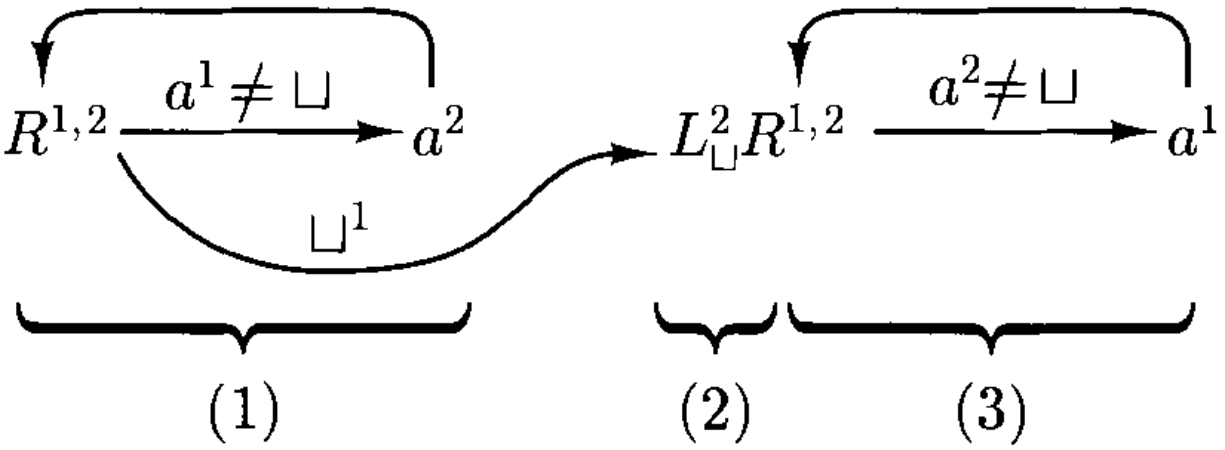
\includegraphics[width=\linewidth]{img/fig-4.15.png}
  \caption{}
  \label{fig:4.10}
\end{figure}

$k$-tape Turing machines are capable of quite complex computational tasks. We shall show next that any $k$-tape Turing machine can be simulated by a single-tape machine. By this we mean that, given any $k$-tape Turing machine, we can design a standard Turing machine that exhibits the same input-output behavior (decides or semidecides the same language, computes the same function).

\vspace*{\fill}
\columnbreak

Such simulations are important ingredients of our methodology in studying the power of computational devices in this and the next chapters. Typically, they amount to a method for mimicking a single step of the simulated machine by several steps of the simulating machine. Our first result of this sort, and its proof, is quite indicative of this line of reasoning.

\begin{theorem}{}
Let $M = (K, \Sigma, \delta, s, H)$ be a $k$-tape Turing machine for some $k \geq 1$. Then there is a standard Thring machine $M' = (K', \Sigma', \delta', s', H)$, where $\Sigma \subseteq \Sigma'$, and such that the following holds:
\begin{quote}
  For any input string $x \in \Sigma^*$, $M$ on input $x$ halts with output $y$ on the first tape if and only if $M'$ on input $x$ halts at the same halting state, and with the same output $y$ on its tape.
\end{quote}
Furthermore, if $M$ halts on input $x$ after $t$ steps, then $M'$ halts on input $x$ after a number of steps which is $O(t \cdot (|x| + t))$.
\end{theorem}

\textit{\textbf{!!} Check the proof of the Theorem 3.1 in the textbook.}

By using the conventions described for the input and output of a $k$-tape Turing machine, the following result is easily derived from the previous theorem.

\begin{formula}{Corollary}
  Any function that is computed or language that is decided or semidecided by a $k$-tape Turing machine is also computed, decided, or semidecided, respectively, by a standard Turing machine.
\end{formula}

\subsection{Two-way Infinite Tape}

Suppose now that our machine has a tape that is infinite in both directions. All squares are initially blank, except for those containing the input; the head is initially to the left of the input. Also, our convention with the $\tar$ symbol would be unnecessary and meaningless for such machines.

It is not hard to see that, like multiple tapes, two-way infinite tapes do not add substantial power to Turing machines. A two-way infinite tape can be easily simulated by a 2-tape machine: 
\begin{itemize}
  \item one tape always contains the part of the tape to the right of the square containing the first input symbol, and 
  \item the other contains the part of the tape to the left of this in reverse.
\end{itemize}
In turn, this 2-tape machine can be simulated by a standard Turing machine. In fact, the simulation need only take linear, instead of quadratic, time, since at each step only one of the tracks is active. Needless to say, machines with several two-way infinite tapes could also simulated in the same way.

\vspace*{\fill}
\columnbreak

\subsection{Multiple Heads}

What if we allow a Thring machine to have one tape, but several heads on it? In one step, the heads all sense the scanned symbols and move or write independently. (Some convention must be adopted about what happens when two heads that happen to be scanning the same tape square attempt to write different symbols. Perhaps the head with the lower number wins out. Also, let us assume that the heads cannot sense each other's presence in the same tape square, except perhaps indirectly, through unsuccessful writes.)

It is not hard to see that a simulation like the one we used for $k$-tape machines can be carried out for Turing machines with several heads on a tape. The basic idea is again to divide the tape into tracks, all but one of which are used solely to record the head positions. To simulate one computational step by the multiple-head machine, the tape must be scanned twice:
\begin{itemize}
  \item Once to find the symbols at the head positions, and 
  \item again to change those symbols or move the heads as appropriate.
\end{itemize}
The number of steps needed is again quadratic, as in Theorem 3.1. The use of multiple heads, like multiple tapes, can sometimes drastically simplify the construction of a Turing machine.

\subsection{Two-Dimensional Tape}

Another kind of generalization of the Turing machine would allow its ``tape'' to be an infinite two-dimensional grid. (One might even allow a space of higher dimension.) Such a device could be much more useful than standard Turing machines to solve problems such as ``zigsaw puzzles''. Once again, however, no fundamental increase in power results. Interestingly, the number of steps needed to simulate $t$ steps of the two-dimensional Turing machine on input $x$ by the ordinary Turing machine is again polynomial in $t$ and $|x|$.

\noindent\rule{\linewidth}{1pt}

The above extensions on the Turing machine model can be combined: One 
can think of Turing machines \textit{with several tapes}, \textit{all or some of which are two-way infinite and have more than one head on them}, or are \textit{even multidimensional}. Again, it is quite straightforward to see that the ultimate capabilities of the Turing machine remain the same.

We summarize our discussion of the several variants of Turing machines discussed so far as follows. 

\begin{theorem}{}
Any language decided or semidecided, and any function computed by Turing machines with several tapes, heads, two-way infinite tapes, or multi-dimensional tapes, can be decided, semidecided, or computed, respectively, by a standard Turing machine.
\end{theorem}

\vspace*{\fill}
\newpage
